%; whizzy paragraph -pdf xpdf -latex ./whizzypdfptex.sh
%; whizzy-paragraph "^\\\\begin{frame}\\|\\\\emtext"
% latex beamer presentation.
% platex, latex-beamer でコンパイルすることを想定。

%     Tokyo Debian Meeting resources
%     Copyright (C) 2012 Junichi Uekawa
%     Copyright (C) 2016 Nobuhiro Iwamatsu

%     This program is free software; you can redistribute it and/or modify
%     it under the terms of the GNU General Public License as published by
%     the Free Software Foundation; either version 2 of the License, or
%     (at your option) any later version.

%     This program is distributed in the hope that it will be useful,
%     but WITHOUT ANY WARRANTY; without even the implied warreanty of
%     MERCHANTABILITY or FITNESS FOR A PARTICULAR PURPOSE.  See the
%     GNU General Public License for more details.

%     You should have received a copy of the GNU General Public License
%     along with this program; if not, write to the Free Software
%     Foundation, Inc., 51 Franklin St, Fifth Floor, Boston, MA  02110-1301 USA

\documentclass[cjk,dvipdfmx,12pt]{beamer}
\usetheme{Tokyo}
\usepackage{monthlypresentation}

%  preview (shell-command (concat "evince " (replace-regexp-in-string "tex$" "pdf"(buffer-file-name)) "&")) 
%  presentation (shell-command (concat "xpdf -fullscreen " (replace-regexp-in-string "tex$" "pdf"(buffer-file-name)) "&"))
%  presentation (shell-command (concat "evince " (replace-regexp-in-string "tex$" "pdf"(buffer-file-name)) "&"))

%http://www.naney.org/diki/dk/hyperref.html
%日本語EUC系環境の時
\AtBeginDvi{\special{pdf:tounicode EUC-UCS2}}
%シフトJIS系環境の時
%\AtBeginDvi{\special{pdf:tounicode 90ms-RKSJ-UCS2}}

\newenvironment{commandlinesmall}%
{\VerbatimEnvironment
  \begin{Sbox}\begin{minipage}{1.0\hsize}\begin{fontsize}{8}{8} \begin{BVerbatim}}%
{\end{BVerbatim}\end{fontsize}\end{minipage}\end{Sbox}
  \setlength{\fboxsep}{8pt}
% start on a new paragraph

\vspace{6pt}% skip before
\fcolorbox{dancerdarkblue}{dancerlightblue}{\TheSbox}

\vspace{6pt}% skip after
}
%end of commandlinesmall

\newcommand{\textframe}[1]{
	\begin{frame}{}
	\begin{center}
	 {\Huge #1
		  }
	 \end{center}
	 \end{frame}
}


\title{Debian/Ubuntu \\ユーザミートアップ in 札幌}
\author{岩松 信洋}
\date{2016年6月17日}
\logo{
\includegraphics[width=8cm]{image200607/openlogo-light.eps}}

\begin{document}

% https://debianjp.doorkeeper.jp/events/46366

\begin{frame}
\titlepage{}
\end{frame}

\begin{frame}{アジェンダ}

\begin{enumerate}
\item 19:00 -    開会の挨拶 / 小岩さん
\item 19:05 - 19:20 Debian / Ruby 関連で何か / 佐々木さん
\item 19:25 - 19:40 Debian / Raspberrypi 3 の話 / 岩松
\item 19:45 - 20:00 Debianパッケージの “説明文” について / 吉野さん
\item 20:05 - 20:20 Ubuntu 16.04 LTS + LXD 2.0 / 水野さん
\item 20:20 - 20:50 ミートアップタイム
\end{enumerate}

\end{frame}

\begin{frame}{頂いた質問}
\begin{itemize}[<+->]
\item 個々のDebianパッケージのビルドログをどこかで見ることはできるのでしょうか?
\item \url{https://packages.qa.debian.org} または \url{tracker.debian.org/}から参照できます。

\begin{center}
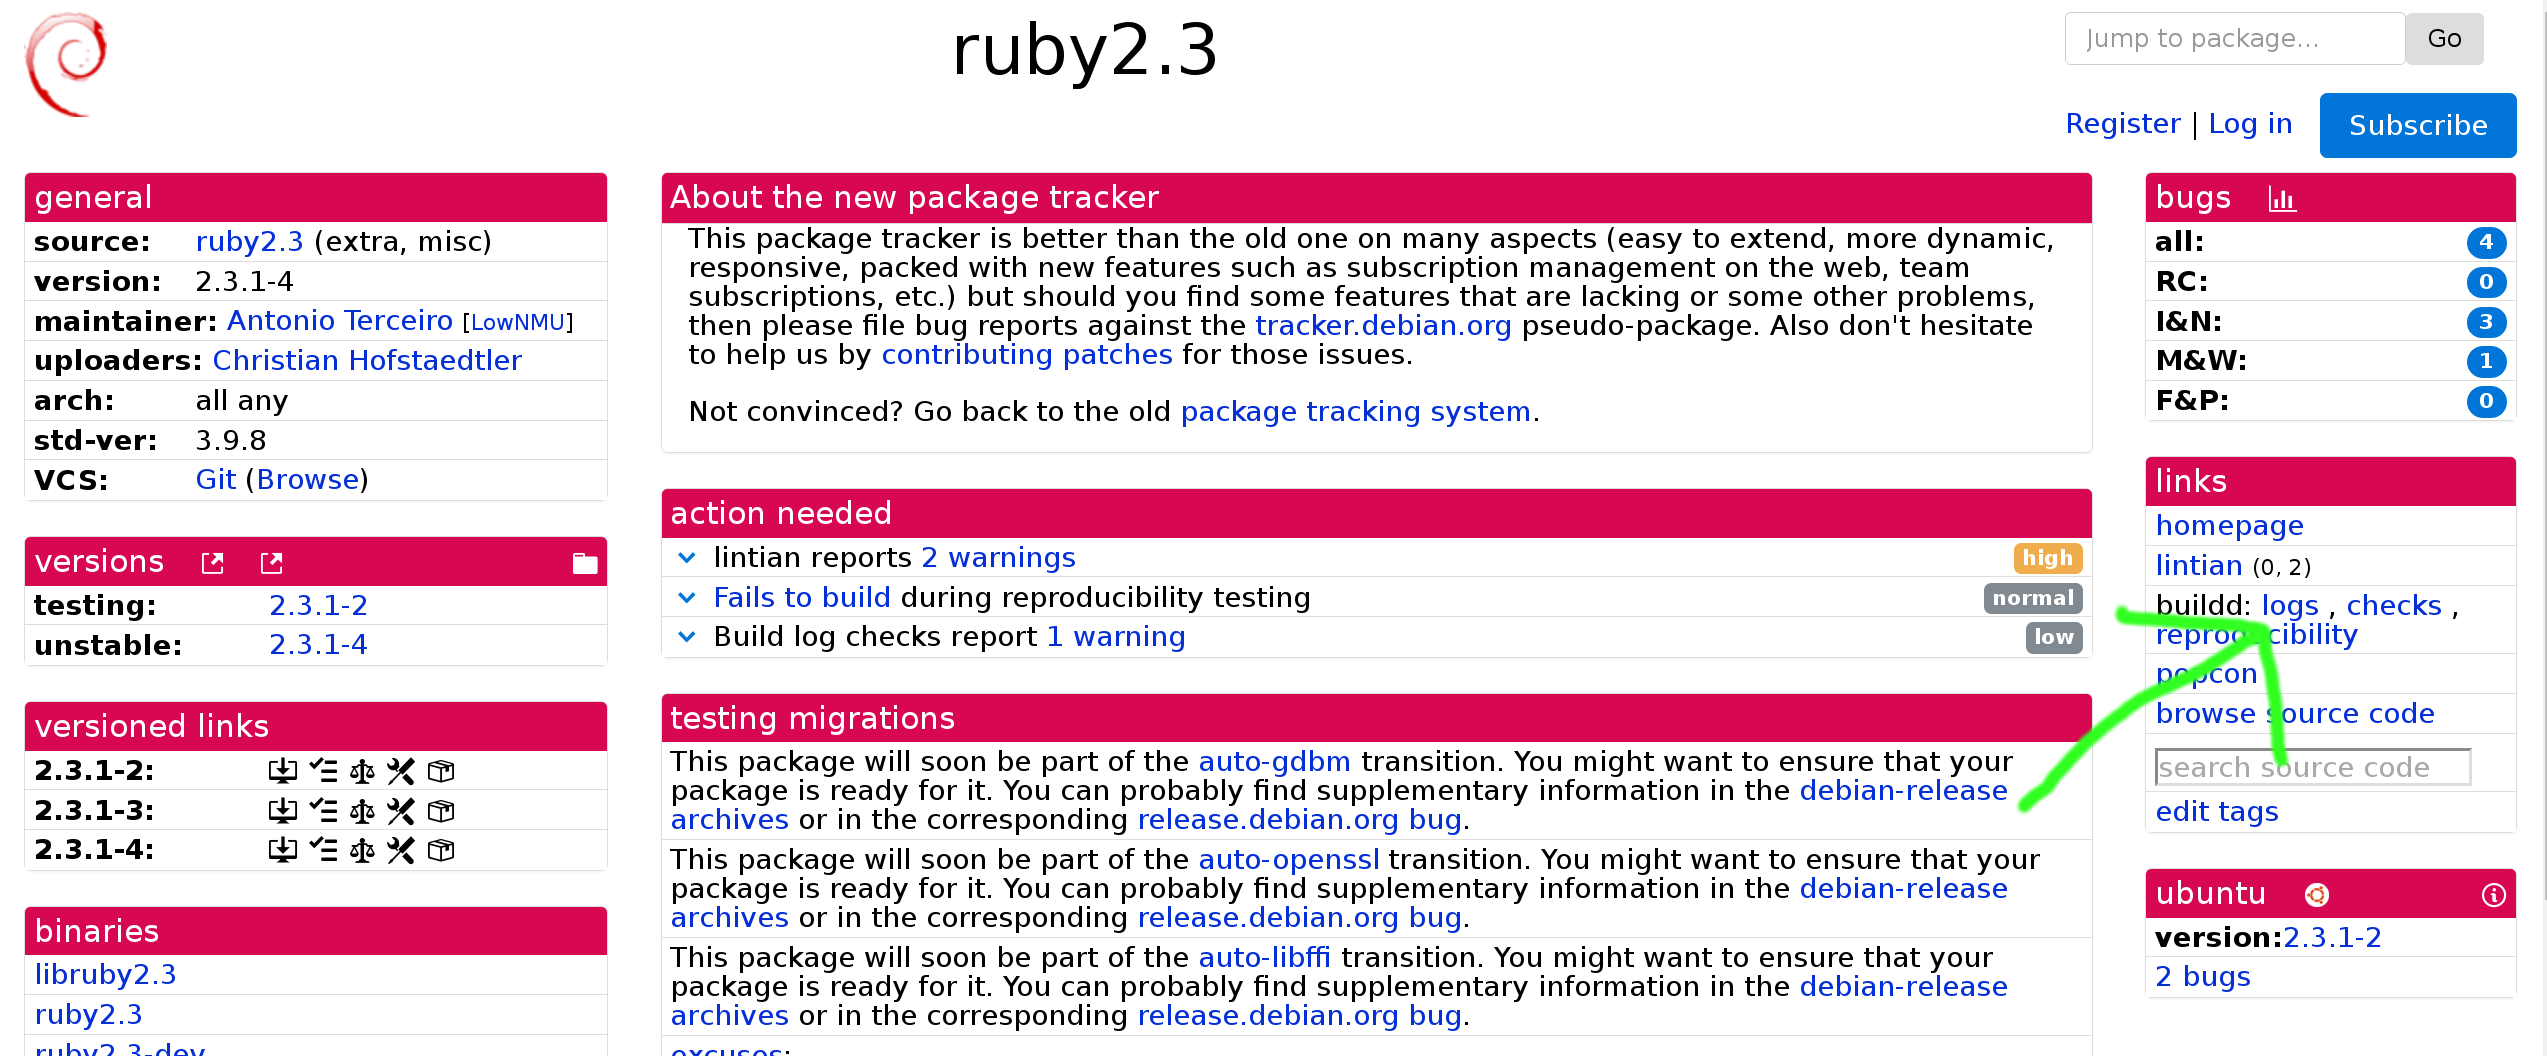
\includegraphics[width=0.8\hsize]{image201606/buildlog0.png}
\end{center}

\end{itemize}
\end{frame}

\begin{frame}{頂いた質問}

\begin{center}
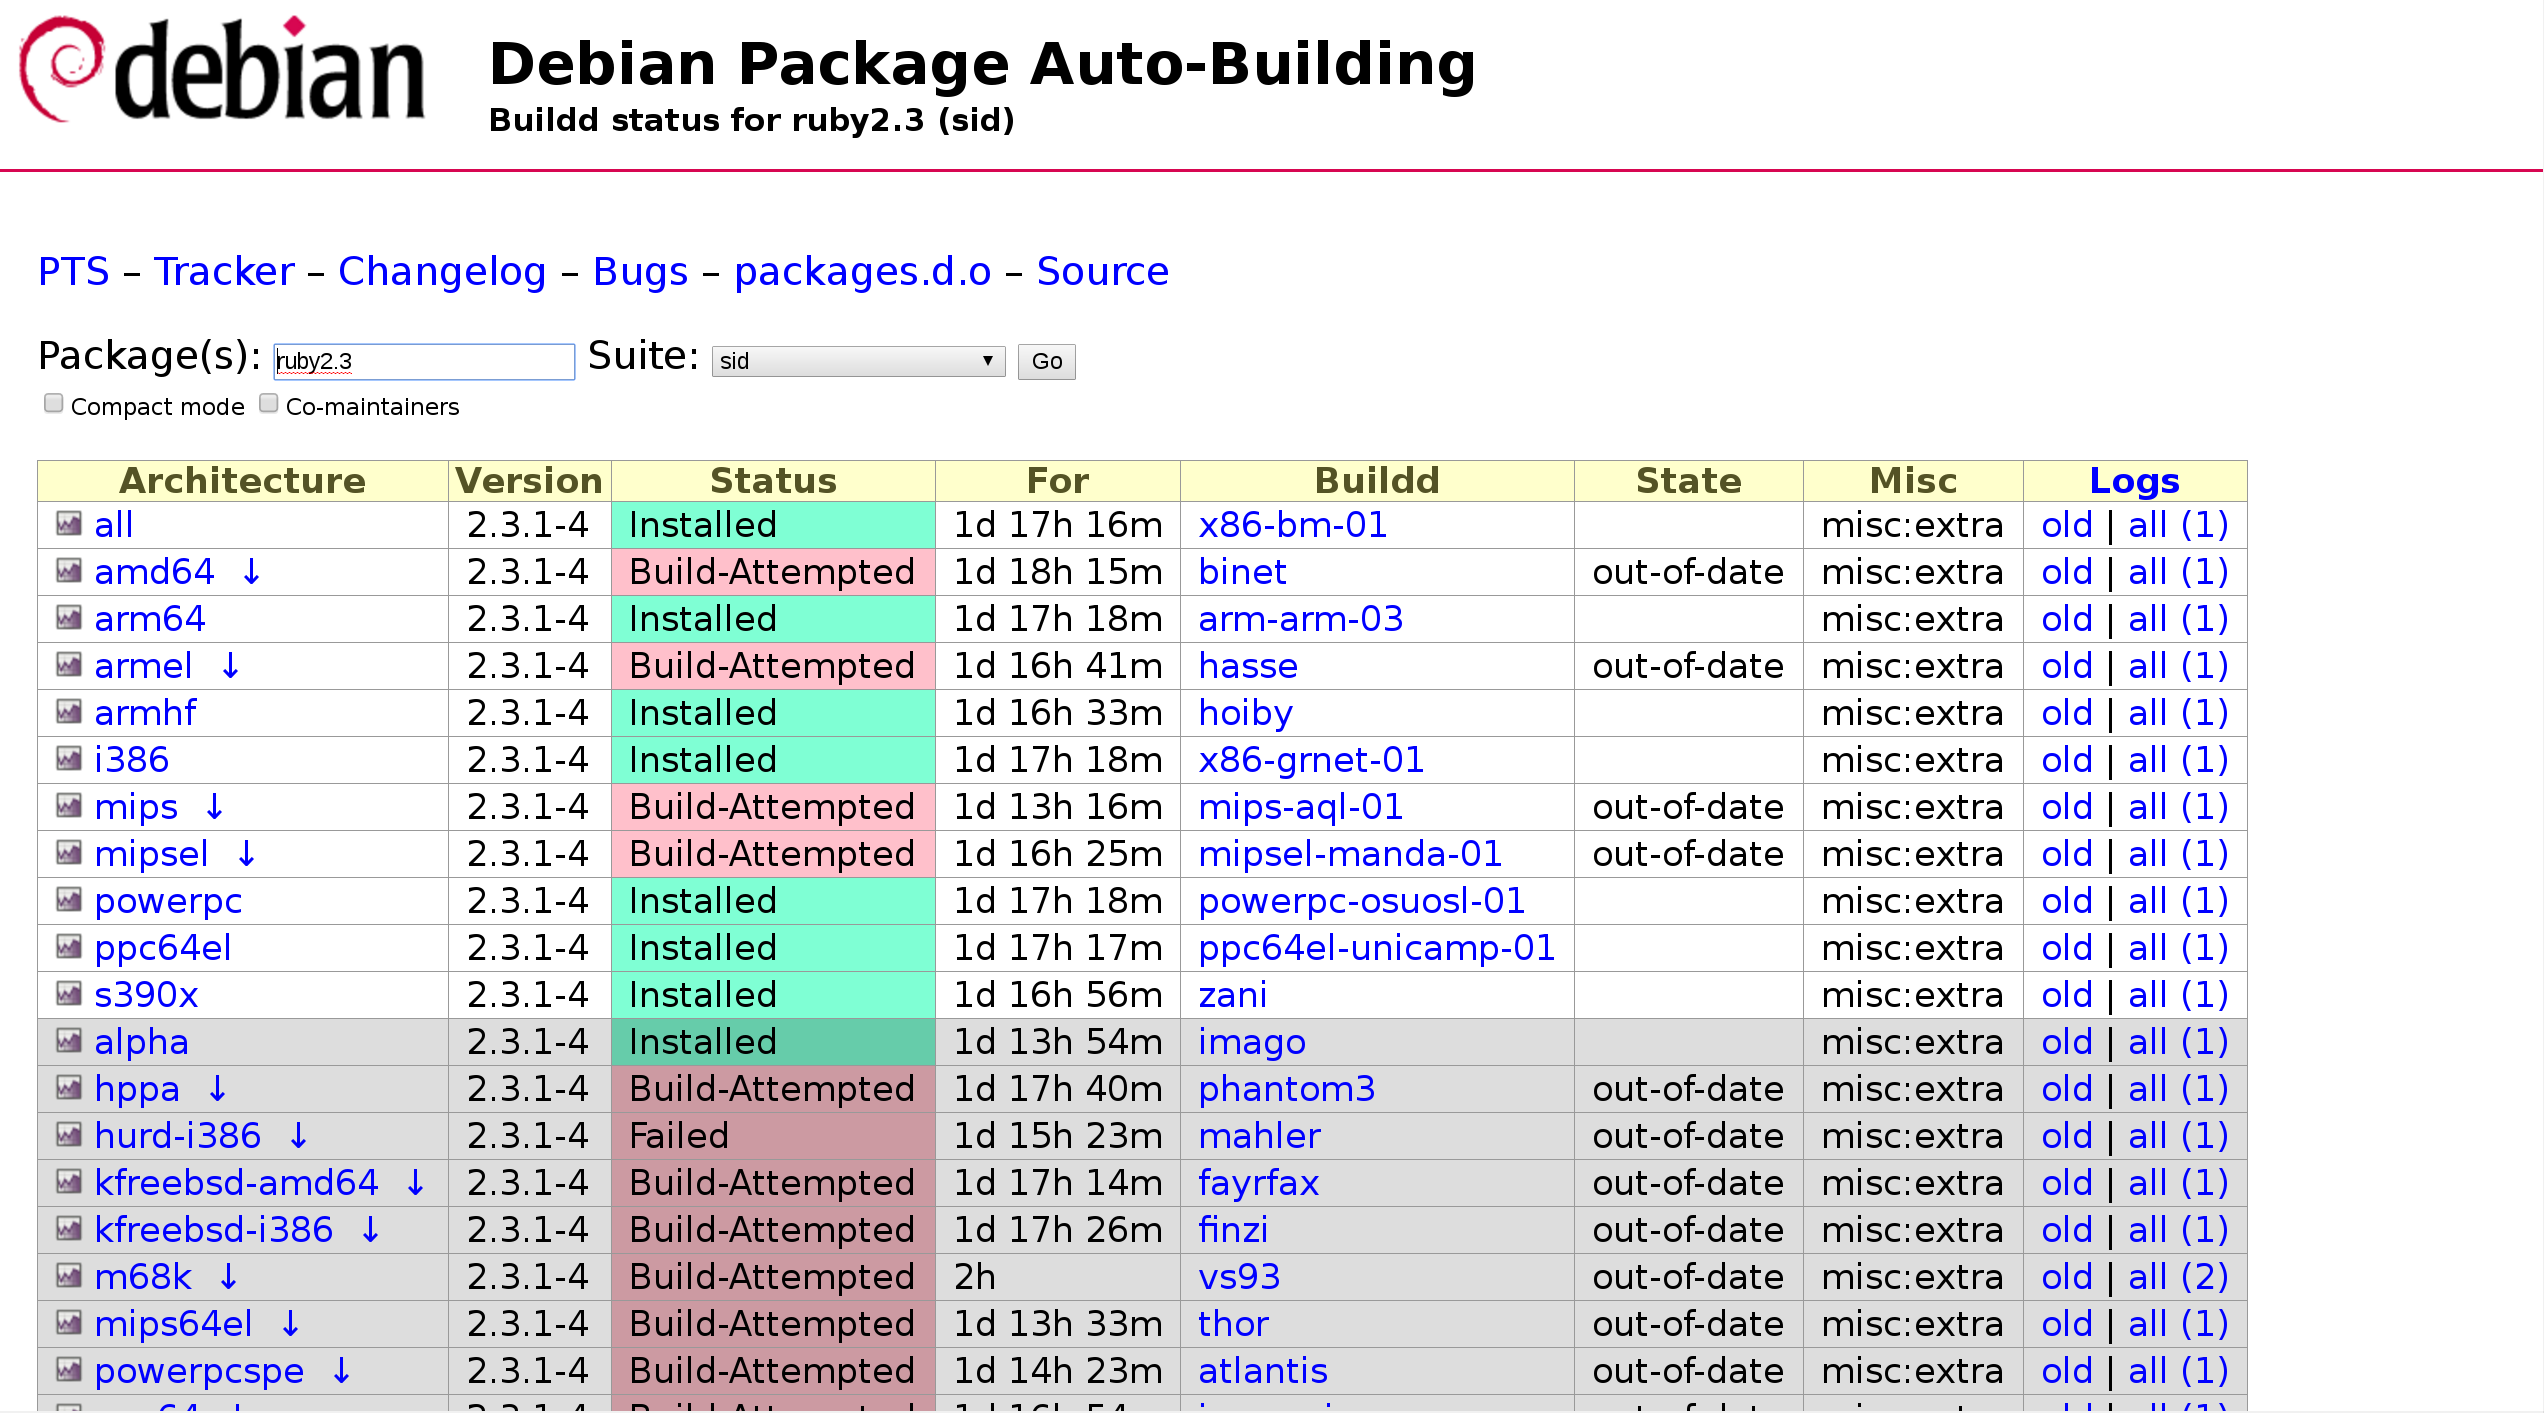
\includegraphics[width=0.8\hsize]{image201606/buildlog1.png}
\end{center}

\end{frame}

\begin{frame}{頂いた質問}
\begin{itemize}[<+->]
\item apache,nginxの設定について聞きたいです。よろしくお願いいたします。
\item apache2 は \url{http://tokyodebian.alioth.debian.org/pdf/debianmeetingresume201203.pdf}
に基本的な使い方がまとまっている。nginx は会場にプロがたくさんいるはず!
\end{itemize}
\end{frame}

\begin{frame}{頂いた質問}
\begin{itemize}[<+->]
\item 個人的にはUbuntuを使いたいのですが、現在会社で使っているリソースがCentOSベースです。個人のわがままな話ですが、どうしたら多大な影響なくUbuntuにシフトできるでしょうか。
\end{itemize}
\end{frame}

\begin{frame}{OSC2016北海道}
\begin{itemize}[<+->]
\item 明日開催される Debian JP Project とUbuntu Japanese Team はセミナーとブース出展しています。
\item 11:00 - Debian Updates
\item 15:15 - Ubuntu 16.04のご紹介
\end{itemize}

\end{frame}

\end{document}

;;; Local Variables: ***
;;; outline-regexp: "\\([ 	]*\\\\\\(documentstyle\\|documentclass\\|emtext\\|section\\|begin{frame}\\)\\*?[ 	]*[[{]\\|[]+\\)" ***
;;; End: ***
